\subsection{Technischer Ablauf der Visualisierung}
\label{subsec:technische-details-zur-visualisierung}


Im folgenden Unterkapitel wird der Ablauf des Erstellens der Tabelle für die in der Datenbank enthaltenen Berichte, so wie die
Erstellung der Graphen grob beschrieben und ein Beispiel der Ergebnisse gegeben.

\subsubsection{Erstellen der Berichtstabelle}

Das Erstellen der Berichtstabelle für die Seite „Report-Tabelle“ läuft wie folgt ab:

\begin{enumerate}

    \item Beim Laden der Seite oder beim Bestätigen bzw. Zurücksetzen der Filterbedingungen wird die Funktion \code{report()} der Seite ausgeführt.
    Diese übermittelte die Filterinhalte über die GET-Methode an die Funktion \code{query\_reports()} aus der Datei \code{queries.py}.
    Diese Funktion führt über \code{db} einen SELECT-Befehl über die Reportdaten aus, welche die Filterbedingungen erfüllen.
    \item Die ausgewählten Datensätze werden nach Rp\_id geordnet und an die Funktion \code{report()} aus der Route-Datei der Seite zurückgegeben.
    Die Datei \code{route.py} ist für die Veranschaulichung in Abbildung \ref{fig:Code routes.py aus Report-Tabellen-Seite} dargestellt.
    \item Diese Funktion lädt das Template der Seite neu und übergibt die ausgewählten Datensätze.
    \item Durch das erneute Laden wird mittels der HTML-Datei \code{reports.html} und der JavaScript-Datei \code{datatable.js} eine Tabelle mit den
    ausgewählten Datensätzen erstellt.

\end{enumerate}

\begin{figure}[H]
    \centering
    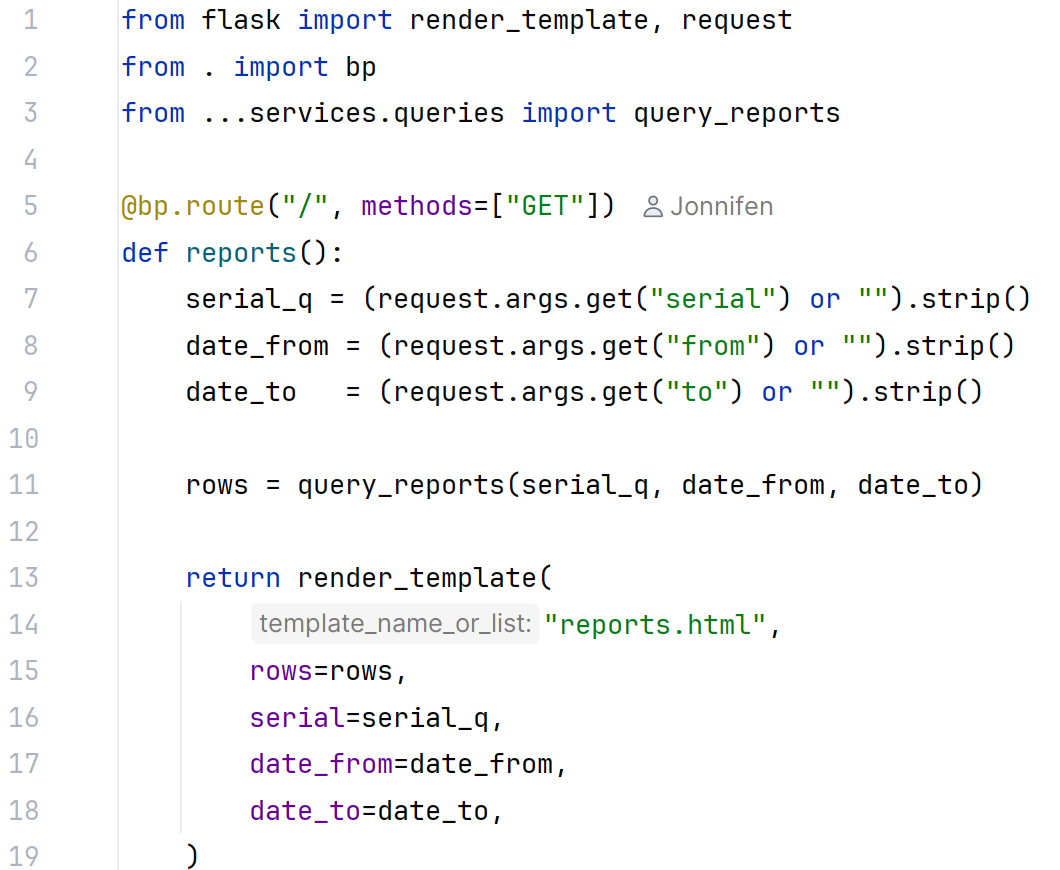
\includegraphics[width=1\textwidth]{Grafiken/route-reports}
    \caption{Code routes.py aus Report-Tabellen-Seite}
    \label{fig:Code routes.py aus Report-Tabellen-Seite}
    {Quelle: Eigene Darstellung}
\end{figure}

Dieser Ablauf wird jedes Mal, wenn die Seite geladen oder z. B. durch das Ändern der Filterbedingungen refreshed wird, durchgeführt.
Nach dem Laden der Seite für die Report-Tabelle werden erst alle in der Datenbank enthaltenen Berichte ausgegeben, bis Filterargumente festgelegt und bestätigt werden.
Ein Ausschnitt dieser Tabelle ist in Abbildung \ref{fig:Ausschnitt der Report-Tabelle} dargestellt.

\begin{figure}[H]
    \centering
    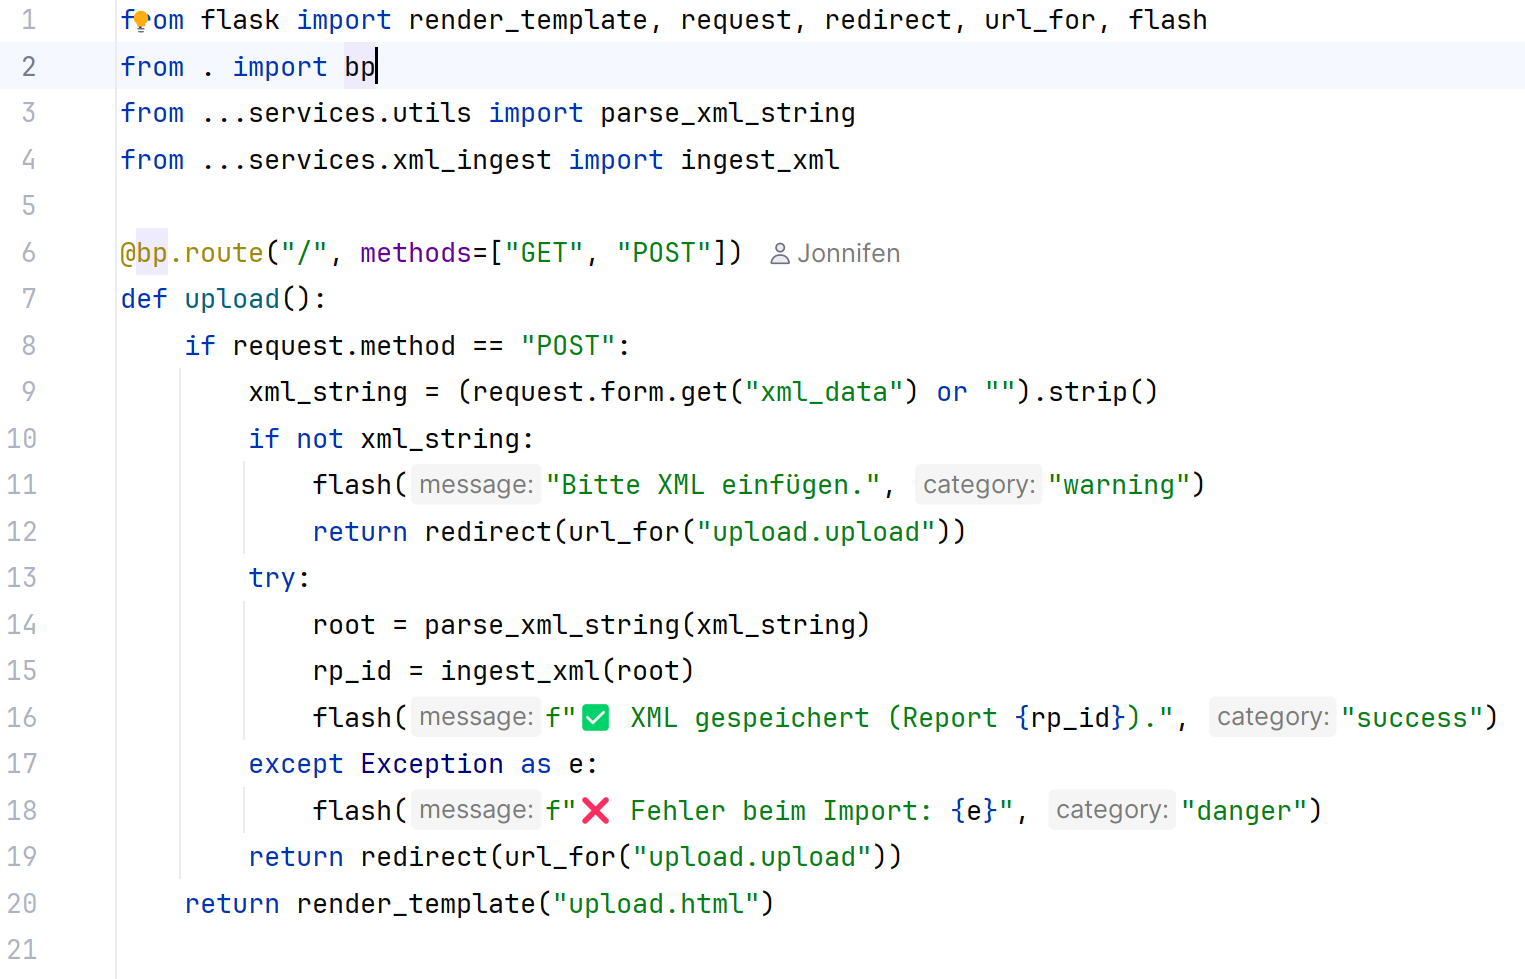
\includegraphics[width=1\textwidth]{Grafiken/Code route Up}
    \caption{Ausschnitt der Report-Tabelle}
    \label{fig:Ausschnitt der Report-Tabelle}
    {Quelle: Eigene Darstellung}
\end{figure}

\subsubsection{Erstellen der Messwert-Graphen}

Das Erstellen der Graphen ähnelt vom grundlegenden Ablauf her der Seite „Report-Tabelle“.
Der Ablauf für das Erstellen der Graphen der Analyse-Seite läuft wie folgt ab:

\begin{enumerate}

    \item Die Variablen zum Finden des gesuchten \ac{DUTs} können über das Eingeben der in die Suchfelder auf der Analyse-Seite
    oder über Links in der Tabelle auf der Seite der Report-Tabelle eingetragen werden.
    Das Laden dieser Variablen geschieht über die GET-Methode.
    und wird über die Funktion \code{dut\_root()} aus der Route-Datei für die Analyse-Seite durchgeführt.
    \item Die Funktion \code{dut\_root()} führt über \code{db} SELECT-Befehle aus, um die notwendigen Datensätze für die darzustellenden Testmodule (PulsTest und XPowerTest) zu erhalten.
    Hierfür werden Funktionen, unter anderem die Funktion \code{get\_series\_vals\_and\_unit()} aus \code{queries.py}, verwendet, um Datensätze zu suchen.
    Für eine Darstellung der Funktion siehe Abbildung \ref{fig:Beispielcode einer Such-Funktion}.
    \item Die ausgewählten Datensätze werden noch geordnet und am Ende lädt die Funktion die Seite neu.
    \item Beim Neuladen werden die Daten an die HTML-Datei \code{dut\_analyse.html} weitergegeben.
    In dieser werden die geordneten Datensätze mit Hilfe der JavaScript-Dateien \code{dut\_plot.js} und \code{plotly-latest.min.js} verarbeitet und die Graphen für die Analyse-Seite erstellt und ausgegeben.

\end{enumerate}

\begin{figure}[H]
    \centering
    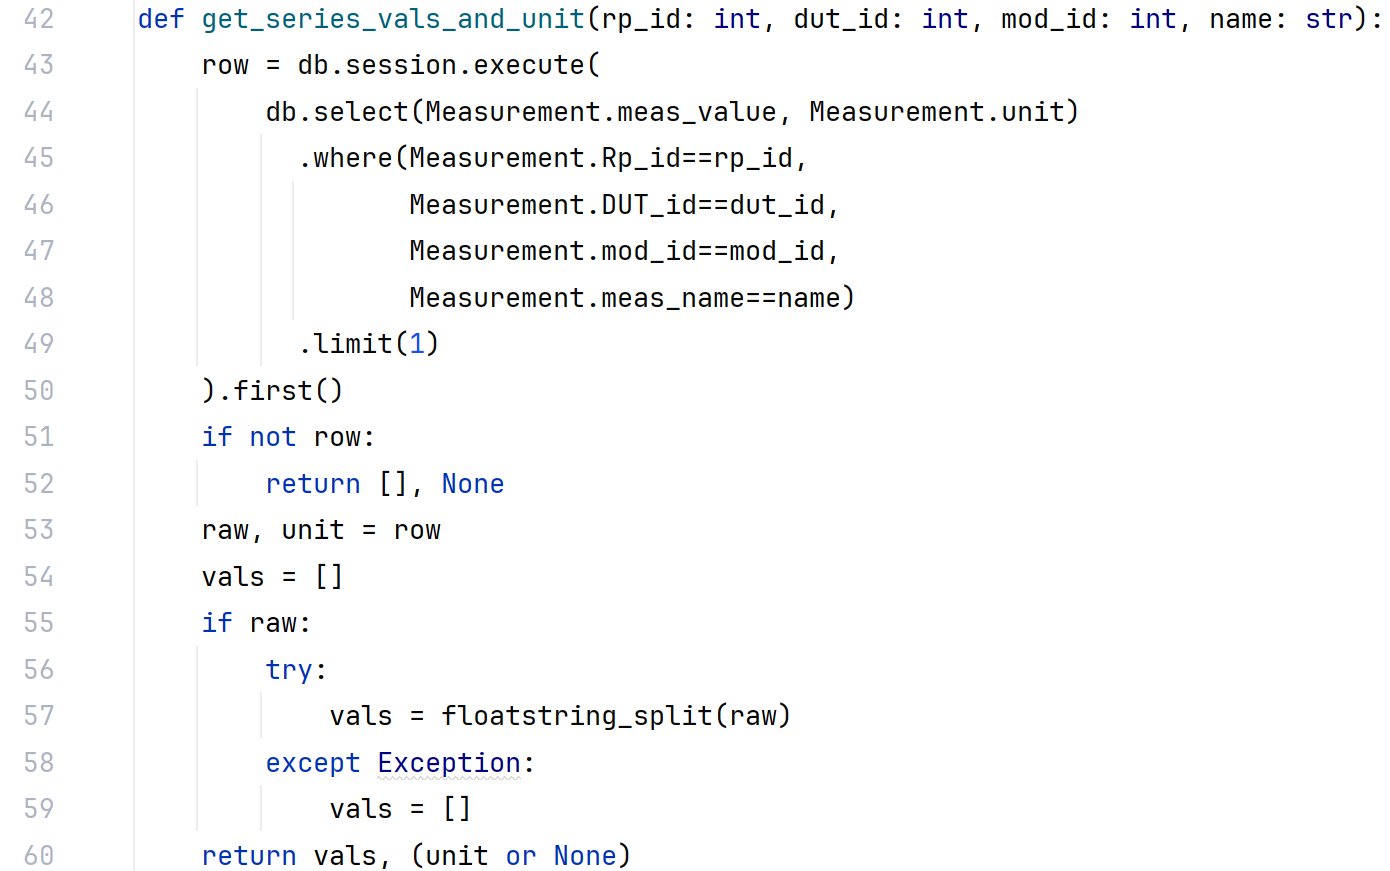
\includegraphics[width=1\textwidth]{Grafiken/get-series.png}
    \caption{Beispielcode einer Such-Funktion}
    \label{fig:Beispielcode einer Such-Funktion}
    {Quelle: Eigene Darstellung}
\end{figure}

Dieser Ablauf wird jedes Mal, wenn die Seite geladen oder z. B. durch das Ändern der Suchbedingungen refreshed wird, durchgeführt.
In der Folge sind zwei auf diese Weise erstellte Graphen dargestellt.
In Abbildung \ref{fig:Beispiel-Graph für PulsTest-Daten} ist ein Graph für die Darstellung der PulsTest-Daten dargestellt.
Die Abbildung \ref{fig:Beispiel-Graph für XPowerTest-Daten} ist ein Graph für die Darstellung der XPowerTest-Daten.

\begin{figure}[H]
    \centering
    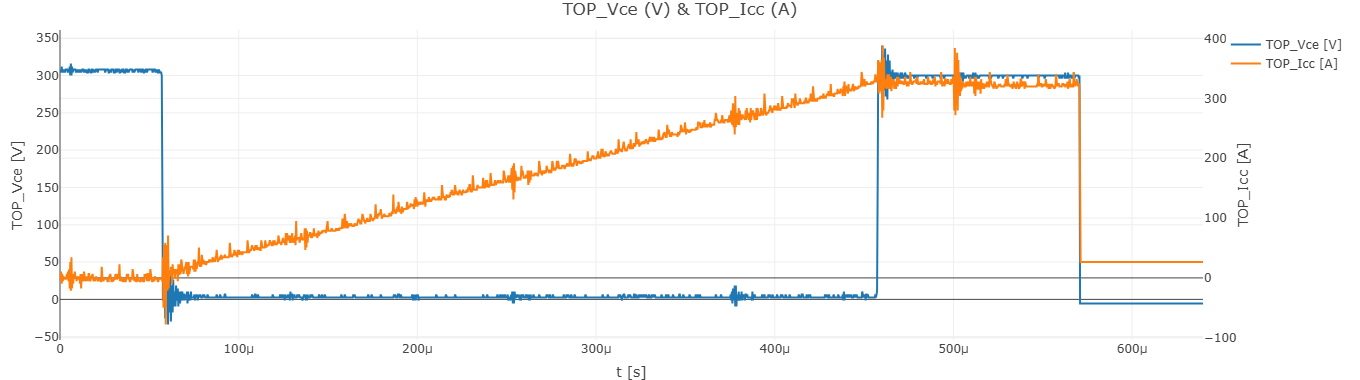
\includegraphics[width=1\textwidth]{Grafiken/newplot.png}
    \caption{Beispiel-Graph für PulsTest-Daten}
    \label{fig:Beispiel-Graph für PulsTest-Daten}
    {Quelle: Eigene Darstellung}
\end{figure}

\begin{figure}[H]
    \centering
    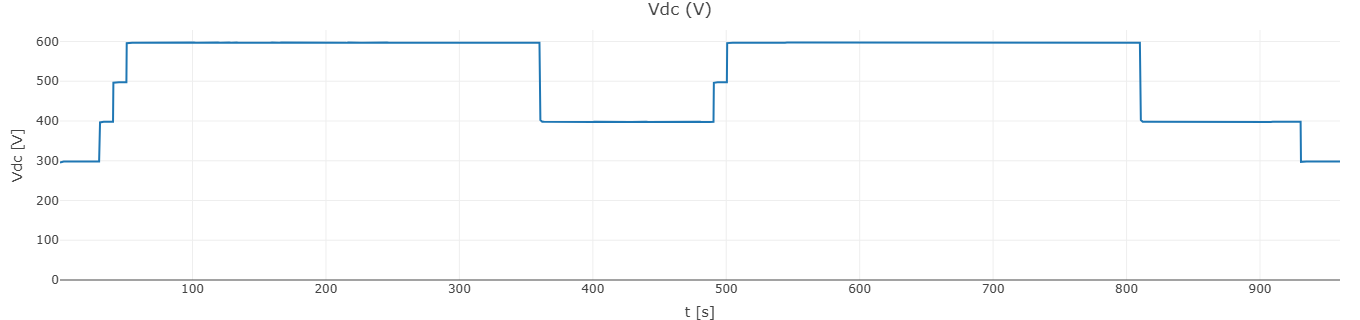
\includegraphics[width=1\textwidth]{Grafiken/newplot (1).png}
    \caption{Beispiel-Graph für XPowerTest-Daten}
    \label{fig:Beispiel-Graph für XPowerTest-Daten}
    {Quelle: Eigene Darstellung}
\end{figure}

Die auf diese Weise erstellten Graphen wurden mit den späteren Nutzern überarbeitet, um die fachgerechte Darstellung und Benennung der Graphen zu gewährleisten.

